\chapter{Model checking for Markov decision processes}

Storm allows to model-check discrete-time and continuous-time models, i.e.,
verify that properties hold in states of models. This
chapter will cover discrete-time model checking via a \textit{probabilistic branching-time logic}. We will detail the syntax, the semantic and model checking algorithms of this logic.
We will see that it is possible to extend this logic to support weights of MCs and MDPs. Then, we will see that it is
possible to formulate requests with this logic to solve
problems we encountered in the first chapter and that we
will address in the following chapter, covering multi-objective support for MDPs. \\

As model checking for MDPs uses the notion of strategy to resolve nondeterminism,
we first need to introduce the probabilistic branching time logic for MCs.

\section{Probabilistic computational tree logic}
\textit{Probabilistic computational tree logic} (or \textbf{PCTL}, for short) is a \textit{branching-time temporal logic}.
This logic allows to verify probabilistic systems via an
%probabilistic
execution tree, actually named \textit{computational tree}. For a given system, this tree consists of an infinite unfolding of this system, considering
all branching possibilities.
%Thus, it is actually an MC with an infinite tree as underlying graph.
The key idea of this tree is that each branch of a node leads to a possible future of this node.
So, this tree is highly linked to cylinder sets.  Possible futures of a node actually correspond to paths of the cylinder set for which the prefix leads the root to the node in the tree.
\begin{example}[\textit{Computational tree of an MC}]
Let $\mathcal{M}$ be the MC of the figure \ref{ct1}. The computational tree of $\mathcal{M}$ starting from the state $s_0$ is
given in the figure \ref{ct2}. We clearly see in this tree that each possible future of a node $s^*$ actually corresponds to a state $s'_n$ of a path $\pi = s'_0 \dots s'_k \dots s'_n \dots \in Cyl(s'_0 \dots s'_k)$ such that $s'_0 = s_0$, $s'_k=s^*$ and $k < n$.
For example, $s_1$ is a possible future of the node $s_0$ (for which the prefix is $s_0s_0$ in the tree) because the path $\pi = s_0s_0s_0(s_1s_2)^\omega$ is in $Cyl(s_0s_0)$.
\begin{figure}[h]
  \begin{minipage}{0.4\linewidth}
    \centering
    \includegraphics[width=0.8\linewidth]{resources/CLT_unfolding_1}
    \captionsetup{justification=centering}
    \captionof{figure}{MC $\mathcal{M}$ with $3$ states, $s_0, s_1$ and $s_2$, and $2$ atomic propositions, $a$ and $b$}\label{ct1}
  \end{minipage}
  \begin{minipage}{0.6\linewidth}
    \centering
    \includegraphics[width=0.8\linewidth]{resources/CLT_unfolding_2}
    \captionsetup{justification=centering}
    \captionof{figure}{Computational tree of $\mathcal{M}$ starting from $s_0$}\label{ct2}
  \end{minipage}
\end{figure}
We will see that it is possible to express formulae in PCTL describing states properties of the system like the following one:
\begin{center}
``\textit{Do all executions starting from the state $s_0$ always eventually reach $b$ with a nonzero probability ?}''
\end{center}
Model checking algorithms of PCTL will answer \textit{yes} to this.
Intuitively, if we refer to the computational tree,
%we see that it is possible to reach a node labeled with $b$,
%from any node of the tree,
%via a path from this node that has a nonzero probability.
%we see that it is possible to reach a node labelled with $b$ from any node of the tree and, each cylinder set
%for which the prefix leads the root to any node has a nonzero probability:
we see that a node labelled with $b$ appears in the future of any node $s^*$ of the tree. Furthermore, there exists an index $n$ for each path $\pi = s'_0 s'_1 s'_2 \dots s'_n \dots \in Cyl(s'_0 \dots s'_k)$, where $s'_0 \dots s'_k$ is the prefix that leads the root to the node $s^* = s'_k$ in the tree, such that $k <n$ and $s'_n$ is labelled with $b$, except for the path $s_0^\omega$ (corresponding to the left path in the computational tree).
Since this path has a zero probability, we have that this property is verified with a probability one from the state $s_0$.
We will see in this chapter how to verify formally each property of this type.
%let $\hat{\pi} = s'_0 \dots s'_n$ be a finite path of $\mathcal{M}$, starting from the state $s_0$ of $\mathcal{M}$ and referring to a finite path starting from the root of the tree. If there exists an index $k$, such that $1 \leq k \leq n$ and $s'_k = s_1$, then $\mathbb{P}_{s_0}(Cyl(s'_0 \dots s'_k \dots s'_n)) = \prod_{i=0}^{k-1} \Delta(s'_i, s'_{i+1}) \cdot 1^\omega = \frac{1}{10}^{k-1}$.
%Else, $\hat{\pi} = s_0^{n+1}$ and $\mathbb{P}_{s_0}(Cyl(s_0^{n+1})) = \frac{1}{10}^n$.
%Furthermore, all executions starting from $s_0$ has a probability one to always eventually reach a state labeled with $b$: the only path starting from $s_0$ that does not allow it is the path $s_0^\omega$ (corresponding to the left path in the computational tree) and has a zero probability.
\end{example}

\subsection{Syntax and semantic}
PCTL has a two stages syntax where PCTL formulae are classified into state and path formulae. Intuitively, \textit{state formulae} are assertions about atomic propositions in a state $s$ and about probabilities over their branching structure, i.e., probabilities of \textit{path formulae} starting from $s$. Actually, a path formula will impose conditions on a set of paths and this path formula will be quantified
by probability bounds.

\begin{definition}[\textbf{Syntax of PCTL}]
Let $AP$ be a set of atomic propositions,
\begin{itemize}
  \item PCTL \textit{state formulae} are formed according the following grammar:
  \[
    \Phi ::= true \;\; | \;\; a \;\; | \;\; \Phi_1 \wedge \Phi_2 \;\; | \;\; \neg \Phi \;\; | \;\; \mathcal{P}_J(\phi)
  \]
  where $a \in AP$ is an atomic proposition, $J \subseteq [0, 1]$ gives probability bounds and $\phi$ is a path formula.
  \item PCTL \textit{path formulae} are formed according the following grammar:
  \[
  \phi ::= \bigcirc \Phi \;\; | \;\; \Phi_1 \U \Phi_2 \;\; | \;\; \Phi_1 \U^{\leq n} \Phi_2
  \]
  where $\Phi$, $\Phi_1$ and $\Phi_2$ are state formulae and $n \in \mathbb{N}$.
\end{itemize}
\end{definition}
Intuitively, $\mathcal{P}_J(\phi)$ specify that the probability of paths satisfying the path formula $\phi$ must be in the interval $J$. A path formula is formed by temporal operators, like $\bigcirc$ and $\U$, with $\U^{\leq n}$ being $\U$ bounded by a maximum number of steps.  There exists some other linear temporal operators, dealing with paths of the system (cf. figure \ref{ltl}). These operators can be derived from the PCTL grammar:
let $J \in [0, 1]$ giving probability bounds, $\Phi$ be a state formula and $n \in \mathbb{N}$ be a number of steps,

\makeatletter
\newcommand*\bigcdot{\mathpalette\bigcdot@{.5}}
\newcommand*\bigcdot@[2]{\mathbin{\vcenter{\hbox{\scalebox{#2}{$\m@th#1\bullet$}}}}}

\makeatother
\begin{flalign}
  &\bigcdot \; \mathcal{P}_J(\Diamond \Phi) \equiv \mathcal{P}_J(true \U \Phi) \tag{\textit{eventually} probability} \\
  &\bigcdot \; \mathcal{P}_J(\Diamond^{\leq n} \Phi) \equiv \mathcal{P}_J(true \U^{\leq n} \Phi) \tag{\textit{bounded enventually} probability} \\
  &\bigcdot \; \mathcal{P}_J(\Box \Phi) \equiv
    \neg \mathcal{P}_J(\Diamond \neg \Phi)
    \tag{\textit{always} probability}
\end{flalign}

\begin{figure}[h]
  \centering
  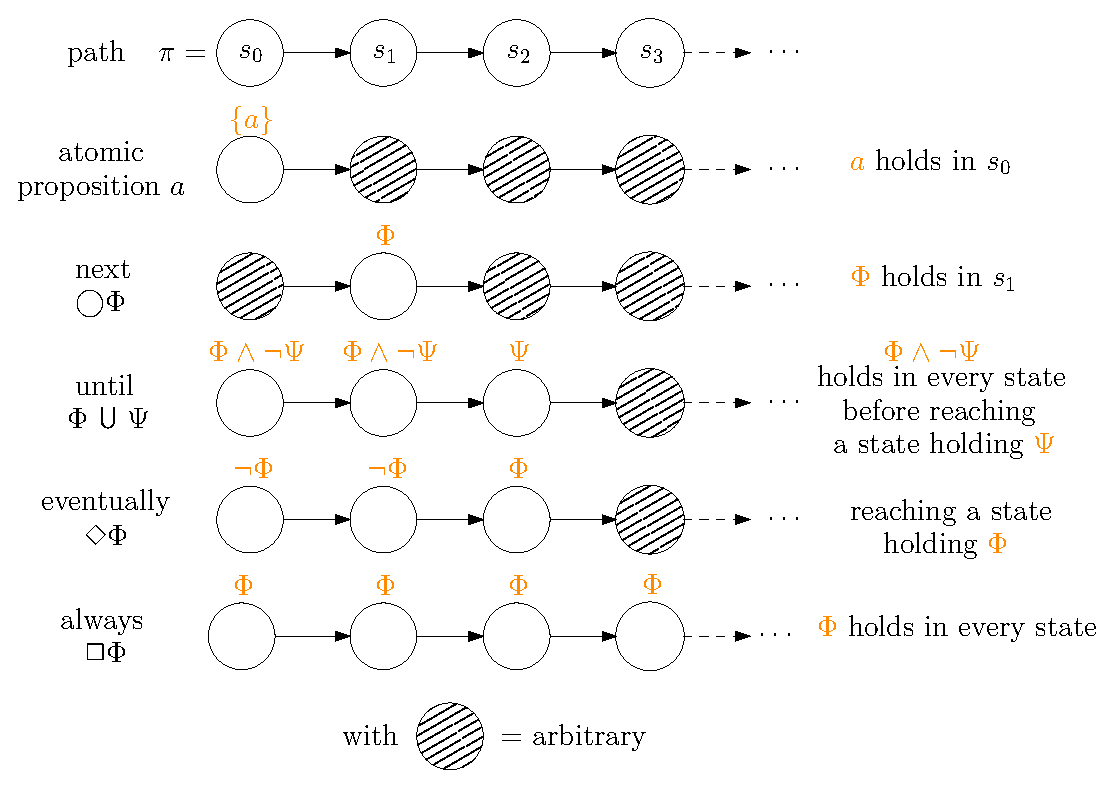
\includegraphics[width=0.85\linewidth]{resources/LTL}
  \caption{Intuitive semantic of linear temporal operators}\label{ltl}
\end{figure}

\begin{definition}[\textbf{Semantic of PCTL}]
  Let $\mathcal{M} = (S, \Delta, AP, L)$ be an MC and $s \in S$, be a state of $\mathcal{M}$,
  \begin{flalign*}
  \intertext{$s \models \Phi$ iff the state formula $\Phi$ holds in the state $s$, i.e.,}
    &\bigcdot\; s \models true, &&&\\
    &\bigcdot\; s \models a &\text{ iff }& a \text{ is a label of $s$, i.e., } a \in L(s),&\\
    &\bigcdot\; s \models \Phi_1 \wedge \Phi_2&\text{ iff }& s \models \Phi_1 \text{ and } s \models \Phi_2,&\\
    &\bigcdot\; s \models \neg \Phi &\text{ iff }& s \not\models \Phi, &\\
    &\bigcdot\; s \models \mathcal{P}_J(\phi) &\text{ iff }& \mathbb{P}_s(\{ \pi \in Paths(s) \; | \; \pi \models \phi \}) \in J.& \\
  \intertext{Following a path $\pi = s_0s_1s_2\dots \in Paths(s)$, $\pi \models \phi$ iff $\pi$ satisfies the path formula $\phi$, i.e., }
  &\bigcdot\;\pi \models \Phi&\text{ iff }&s_0 \models \Phi,&\\
  &\bigcdot\;\pi \models \bigcirc\, \Phi&\text{ iff }&s_1 \models \Phi,&\\
  &\bigcdot\;\pi \models \Phi_1 \U \Phi_2 &\text{ iff }& \exists j \in \mathbb{N},\, s_j \models \Phi_2
    \text{ and } \forall i \in \mathbb{N}, \, i < j, \, s_i \models \Phi_1,&\\
  &\bigcdot\;\pi \models \Phi_1 \U^{\leq n} \Phi_2 &\text{ iff }& \exists j \in \mathbb{N}, \, j \leq n ,\, s_j \models \Phi_2
    \text{ and } \forall i \in \mathbb{N}, \,i < j, \, s_i \models \Phi_1.&\\
  \intertext{Additionally,}
  &\bigcdot\; \pi \models \Diamond \Phi&\text{ iff }& \exists j \in \mathbb{N}, \, s_j \models \Phi,&\\
  &\bigcdot\; \pi \models \Box \Phi&\text{ iff }& \forall j \in \mathbb{N}, \, s_j \models \Phi.&
  \end{flalign*}
\end{definition}
\begin{remark}[\textit{Measurability of path formulae}]
Since $\mathcal{P}_J(\phi)$ refers to probabilities, $\neg \mathcal{P}_J(\phi) = \mathcal{P}_{J'}(\phi)$ for any path formula $\phi$, with $J'=[0, 1] \setminus J$. Then, the event $\{ \pi \in Paths(s) \; | \; \pi \models \phi\}$ must be measurable to verify that $\mathcal{P}_J(\phi)$ holds in any state. We will see that these events can be formed through countable unions of cylinder sets, ensuring their measurability.
\end{remark}
\begin{remark}[\textit{Probabilistic satisfiability of path formulae}]
Let $\mathcal{M}$ be the MC of the figure \ref{pctlctl}.
\begin{figure}[h]
  \centering
  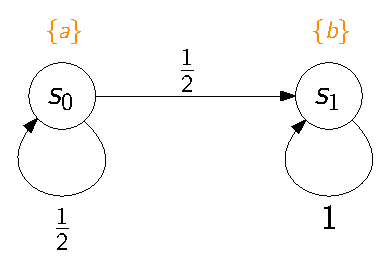
\includegraphics[width=0.25\linewidth]{resources/PCTL_CTL}
  \captionsetup{justification=centering}
  \caption{MC $\mathcal{M}$ with $2$ states, $s_0$ and $s_1$, and $2$ atomic propositions, $a$ and $b$}\label{pctlctl}
\end{figure}
\begin{itemize}
% \item Let assume that there exists a path $\pi \in Paths(s_0)$ starting from $s_0$ in $\mathcal{M}$ such that $\pi \not \models \phi$, for any PCTL path formula $\phi$. That does not mean that $s_0 \models \mathcal{P}_{<1}(\phi)$: take $\pi=s_0^\omega$ and $\phi = \Diamond b$, we have that $s_0^\omega \not \models \Diamond b$ and $\mathbb{P}_s(\Diamond \{s_1\}) = 1$.
% Then $s_0 \models \mathcal{P}_{=1}(\Diamond b)$.
  \item Let assume there exists a state $s$ in an MC such that $s \models \mathcal{P}_{=1}(\phi)$, for any path formula $\phi$. That does not mean that all paths $\pi \in Paths(s)$ satisfy $\phi$, i.e.,
  \[s \models \mathcal{P}_{=1}(\phi) \centernot\implies \forall \pi \in Paths(s), \, \pi \models \phi.\]
  Indeed, consider the MC $\mathcal{M}$ and take the state $s_0$ of $\mathcal{M}$, the path $s_0^\omega \in Paths(s_0)$ and the path formula $\Diamond b$. We have $s_0 \models \mathcal{P}_{=1}(\Diamond b)$, because $\mathbb{P}_{s_0}(\Diamond \{s_1\})=1$, but we have $s_0^\omega \not \models (\Diamond b)$.

  \item Let assume there exists a state $s$ in an MC such that there exists a path $\pi \in Paths(s)$ starting from this state $s$ such that $\pi \models \phi$ for any path formula $\phi$.
  That does not mean that $s \models \mathcal{P}_{> 0}(\phi)$, i.e.,
  \[
    \exists \pi \in Paths(s),\, \pi \models \phi \centernot\implies s \models \mathcal{P}_{>0} (\phi).
  \]
  Indeed, consider the MC $\mathcal{M}$ and take the state $s_0$, the path $s_0^\omega \in Paths(s_0)$ and the path formula $\Box a$. We have that the path $s_0^\omega$ is the only path of $\mathcal{M}$ that verifies $\Box a$ (and thus, $s_0^\omega \models \Box a$).
  However, we have $\mathbb{P}_s(\{s_0^\omega\})=0$. Then, $s_0 \models \mathcal{P}_{=0} (\Box a)$.
\end{itemize}
\end{remark}

\begin{definition}[\textbf{Satisfiability set for PCTL}]
  Let $\mathcal{M}=(S, \Delta, w, AP, L)$ be an MC and $\Phi$ be a PCTL state formula on $AP$. The \textit{satisfiability set} for the MC $\mathcal{M}$ is defined as follows:
  \[
    Sat(\Phi) = \{ s \in S \, | \, s \models \Phi \}.
  \]
\end{definition}

\section{Temporal events in Markov chains}\label{tempevent}
In Markov chains, \textit{temporal events} allow to describe \textit{quantitative} and \textit{qualitative} properties.
Quantitative properties may assert the probability to reach a subset of target states, avoiding some bad states in a infinite or finite number of steps, and
qualitative properties are special cases of quantitative properties where probabilities are trivial (i.e., zero or one).
In order to describe these temporal events, we use \textit{LTL-like} notations.
\textit{Linear temporal logic} (LTL) is a logical formalism
that is suited for specifying linear temporal properties.
In PCTL, notations of linear temporal operators (cf. figure \ref{ltl}) are actually derived from LTL temporal operators, dealing with paths of any system.
For example, following a subset of target states $T \subseteq S$ of the system, the event of reaching $T$ is denoted by $\Diamond T$ that is defined with a finite union of cylinder sets, ensuring its measurability.
We will define here some temporal events, that are actually used to form PCTL path formulae events. So, we need to ensure their measurability.
Furthermore, we will present how to compute their probability, which will be useful later to model-check Markov chains and Markov decision processes in PCTL.
\subsection{Constrained reachability}
\begin{definition}[\textbf{Constrained reachability event}]
Let $\mathcal{M}= (S, \Delta, w, AP, L)$ be an MC, $s \in S$ be a state of $\mathcal{M}$ from which events start, $T, C \subseteq S$ and $n \in \mathbb{N}$.
The events $C \U^{\leq n} T$ and $C \U T$ are defined as follows:
\begin{align*}
  C \U^{\leq n} T &= \bigcup_{k=0}^n\,\bigcup_{s_0\dots s_k \in Paths_{fin}^{C,\, k,\, T}(s)} Cyl(s_0\dots s_k),\\
  C \U T &= \bigcup_{k\in \mathbb{N}}\,\bigcup_{s_0\dots s_k \in Paths_{fin}^{C,\, k,\, T}(s)} Cyl(s_0\dots s_k)
\end{align*}
where \[Paths_{fin}^{C,\, n,\, T}(s) = \{ s_0 \dots s_n \in Paths_{fin}(s) \; | \; s_i \in C\;\; \forall i \in \mathbb{N},\, i < n \; \; \wedge s_n \in T\},\]
and $\mathbb{P}_s(C \U^{\leq n} T), \mathbb{P}_s(C \U T)$ actually denote the probability measure of the union of cylinder sets of finite paths  of $Paths_{fin}^{C, \, k, \, T}(s)$ starting from the state $s \in S$.
\end{definition}

The constrained reachability event allows to derivate some other classical events:
\begin{itemize}
  \item $\Diamond T = S \U T$, i.e., \textit{reach $T$} (cf. subsection \ref{obj-MC} in the first chapter),
  \item $\Box T =  \overline{\Diamond \overline{T}} \; \implies \; \mathbb{P}_s(\Box T) = 1 - \mathbb{P}_s (\Diamond (S \setminus T))$, i.e., \textit{always encounter $T$}.
\end{itemize}
So, if we can compute the constrained reachability event probability, then we are able to compute the probability of $\Diamond T$ and $\Box T$ events.
Let $S_{=0}$, $S_{=1}$ and $S_{=?}$ be partitions of $S$ such that
\begin{itemize}
  \item $T \subseteq S_{=1} \subseteq \{s \in S \; | \; \mathbb{P}_s(C \U T) = 1\}$,
  \item $S \setminus (C \cup T) \subseteq S_{=0} \subseteq \{ s \in S \; | \; \mathbb{P}_s(C \U T) = 0 \}$,
  \item $S_? = S \setminus (S_{=1} \cup S_{=0})$.
\end{itemize}
Then, let $A$ be a quadratic matrix with rows and columns referring the states of $S_?$. This matrix is obtained from the transition function $\Delta$ as follows:
\[
  A_{i, j} = \Delta(s_i, s_j) \quad \forall s_i, s_j \in S_?
\]
Let $n_?$ = $|S_?|$. Similarly, let $b$ be a vector of probabilities in $[0, 1]^{n_?}$ , defined as $(b_s)_{s \in S_?}$ such that $b_s = \sum_{t \in S_{=1}} \Delta(s, t)$, i.e., such that $b_s$ describes the probability of reaching a state of $T$ in one outgoing transition of the state $s$.

\begin{notation}[\textit{Lifted probability transition}]
  Let $s \in S$ be a state of $\mathcal{M}$. We denote by $\Delta(s, T)$ the probability of reaching $T$ in one outgoing transition of $s$, i.e., $\Delta(s, T) = \sum_{t \in T} \Delta(s, t)$.
\end{notation}
\noindent So, we have $b_s = \Delta(s, S_{=1})$ for each $s \in S_?$.
\begin{theorem}[\bfseries\itshape Least fixed point characterisation]\label{theoCUT}
  Let $x$ be a vector of probabilities in $[0,1]^{n_?}$ such that $x=(\mathbb{P}_s(C \U T))_{s \in S_?}$. This vector is the
  \textit{least fixed point} of the operator $\Upsilon : [0, 1]^{n_?} \rightarrow [0, 1]^{n_?}$. Let $(y_s)_{s \in S_?} \in [0, 1]^{n_?}$, the least fixed point of the operator $\Upsilon$ is given by
  \[
    \Upsilon(y) = A y + b
  \]
  Furthermore, let $x^{(0)} = \vec{0}$ be the vector consisting of zeros only and $x^{(n+1)} = \Upsilon(x^{n})$ for $n \in \mathbb{N}$, then
  \begin{itemize}
    \item $x^{(n)} = (x_s^{(n)})_{s \in S_?}$, where $x_s^{(n)} = \mathbb{P}_s(C \U^{\leq n} S_{=1})$ for each state $s \in S_?$,
    \item $x^{(0)} \leq x^{(1)} \leq x^{(2)} \leq \dots \leq x$, and
    \item $x = \lim_{n\rightarrow\infty}x^{(n)}$.
  \end{itemize}
  where $\leq$ denotes here the partial order relation \[\leq \,=\, \{ (y, y') \in [0, 1]^{n_?} \times [0,1]^{n_?} \; | \; y_s \leq y'_{s} \;\; \forall s \in S_?\}.\]
\end{theorem}
By definition of $A$ and $b$, for any $s \in S_?$ and for $y = (y_s)_{s \in S_?}$,
\[
  (\Upsilon(y))_s = y_s = \sum_{s' \in S_?} \Delta(s, s') \cdot y_{s'} + \Delta(s, S_{=1}).
\]
Furthermore, let $x_s = \mathbb{P}_s(C \U T)_{s \in S_?}$ for each state $s \in S$, by definition of $\Upsilon$, we have that
\begin{flalign}
  x^{(0)} &= \vec{0}, \notag \\
  x^{(1)} &= A x^{(0)} + b \notag \\
          &= b, \tag{\itshape state of $C$ reaching $S_{=1}$ in one transition}\\
  x^{(2)} &= A x^{(1)} + b \notag \\
          &= A b + b \notag \\
          &= (\sum_{s' \in S_?} \Delta(s, s') \cdot \Delta(s', S_{=1}) + \Delta(s, S_{=1}))_{s \in S_?} \tag{\itshape state of $C$ reaching $S_{=1}$ in max. two transition steps} \\
  &\dots \notag \\
  x^{(n)} &= A x^{(n-1)} + b \tag{\itshape state of $C$ reaching $S_{=1}$ in max. $n$ transition steps} \\
  &\dots \notag \\
  x &= Ax+b \notag \\
  x &= (\sum_{s' \in S} \Delta(s, s') \cdot x_{s'} + \Delta(s, S_{=1}))_{s \in S_?} \tag{\itshape state of $C$ eventually reaching $S_{=1}$}
\end{flalign}
\begin{remark}[\textit{Choosing $S_{=0}$ and $S_{=1}$}]\label{remarkS0S1}
For efficiency reasons, it is a good idea to deal with the largest subsets $S_{=0}$ and $S_{=1}$. Indeed, this allows to reduce
the size of the matrix $A$ and allows faster computations to solve the linear equation defined by $x = Ax + b$.
However, for computational reasons, we need to deal with the largest set $S_{=0}$ as possible, i.e., $S_{=0} = \{ s \in S \; | \; \mathbb{P}_s(C \U T) = 0 \}$. Indeed, for some instance, choosing $S_0 = S \setminus (C \cup T)$ is not sufficient.
Let $\mathcal{M}$ be the MC of the figure \ref{s0s1} and $T = \{t\}$.
\begin{figure}[h]
  \centering
  \includegraphics[width=0.3\linewidth]{resources/S0S1}
  \caption{Markov chain $\mathcal{M}$ with $2$ states : $s$ and $t$}\label{s0s1}
\end{figure}
Consider the event $\Diamond T$. Let take the smallest subsets $S_{=1} = T$ and $S_{=0} = S \setminus (S \cup T) = \emptyset$, thus $S_? = S \setminus T = \{s\}$. Following the theorem \ref{theoCUT}, let $x = (\mathbb{P}_s(C \U T))_{s \in S_?}$, where $x = Ax+b$. As $x=x_s$ and $b = 0$ (because $\Delta(s, t) = 0$),
we have $x = Ax$, with $A = 1$ (because $\Delta(s, s) = 1$). The related operator $\Upsilon:[0, 1] \rightarrow [0,1]$ is given by $\Upsilon(y_s) = y_s$ for any $y_s \in [0, 1]$ and has then infinitely many fixed points.
\end{remark}
% \begin{definition}[\textbf{Paths satisfiability of $C \U T$ events}]
%   Let $\mathcal{M}=(S, \Delta, w, AP, L)$ be an MC, $T, C \subseteq S$ and $\pi \in Paths(s)$ be a path starting from any $s \in S$. The path $\pi$ satisfies the event $C \U T$ iff
% \end{definition}
Unique fixed point is actually guaranteed if $\mathcal{M}$ is finite and if we take the largest subset for $S_{=0}$, i.e., $S_{=0}=\{s \in S \; | \; \mathbb{P}_s(C \U T) =0 \}$. We will now provide a way to compute this subset.
\begin{definition}[\textbf{Path satisfiability relation of constrained reachability events}]
Let $\mathcal{M}$ be an MC with state space $S$ and $\pi \in Paths(s)$ be a path starting from any state $s \in S$. The path $\pi$ \textit{satisfies} $C \U T$ iff there exists a prefix $\hat{\pi}\in pref(\pi)$ and a number of steps $k \in \mathbb{N}$ such that $\hat{\pi} \in Paths_{fin}^{C,\, k,\, T}(s)$. This relation is denoted by $\models$, with $\pi \models C \U T$.
\end{definition}
\begin{lemma}[Zero probability equivalence of constrained reachability events] Let $s \in S$ be a state in an MC with state space $S$ and $C, T \subseteq S$, the two following propositions are equivalent:
  \begin{enumerate}[(a)]
    \item $\mathbb{P}_s(C \U T) = 0$ \label{p1}.
    \item $\forall \pi \in Paths(s), \, \pi \not \models (C \U T)$ \label{p2}.
  \end{enumerate}
\end{lemma}

 \begin{proof2}$ $\\
    ($\ref{p2}\implies\ref{p1}$). Let assume that $\forall \pi \in
    Paths(s)$, $\pi \centernot\models C \U T$. So, by definition of the satisfaction relation $\models$, that
    means there does not exist finite path $\hat{\pi} \in
    Paths_{fin}(s)$ and a number of steps $k \in \mathbb{N}$ such that
    $\hat{\pi} \in Paths_{fin}^{C, \, k,\, T}(s)$. By definition
    of $C \U T$, that implies $C \U T = \emptyset$ and then
    $\mathbb{P}_s(\emptyset) = 0$.\\
    ($\neg\ref{p2}\implies\neg\ref{p1}$). Let assume there exists a path $\pi \in Paths(s)$ such that $\pi \models C \U T$.
    Then, that means there exists a prefix $\hat{\pi} = s_0 \dots s_k \in pref(\pi)$ and a number of steps $k \in \mathbb{N}$ such that
    $\hat{\pi} \in Paths_{fin}^{C, \, k, \, T}(s)$. So, we have at least one cylinder set in the union forming the event $C \U T$ (i.e., $Cyl(s_0\dots s_k)$), and then $\mathbb{P}_s(C \U T) \geq \prod_{i = 0}^{k-1} \Delta(s_i , s_{i+1}) > 0$.
 \end{proof2}

\begin{lemma}[Computing $S_{=0}$ with graph theory]\label{S0graph}
Let $s \in S$ be a state in an MC with state space $S$ and $C, T \subseteq S$,
  the statement $\forall \pi \in Paths(s), \, \pi \centernot \models (C \U T)$ can be decided in polynomial time in the size of $\mathcal{M}$ with a graph theory based algorithm.
\end{lemma}

\begin{proof2}
The set $B = \{ s \in S \; | \; \exists \pi \in Paths(s), \;\; \pi \models (C \U T) \}$ is the smallest subset of $S$ such that
\begin{itemize}
  \item $T \subseteq B$, and
  \item $\forall s \in S, \; s \in C \; \wedge \; Succ(s) \cap B \neq \emptyset \implies s \in B$.
\end{itemize}
Indeed,
\begin{enumerate}
  \item Let assume that $B = \{s \in S \; | \; \exists \pi \in Paths(s), \; \pi \models C\U T\}$. We obviously have that $T \subseteq B$ because all path starting from $t \in T$ satisfies $C \U T$: take the finite path consisting in the single state $t$, we have that
  $t \in Paths_{fin}^{C, \, 0,\, T}(t)$. Then, let $s \in S$. Let assume that $s \in C$ and $Succ(s) \cap B \neq \emptyset$. That means there exists a successor $s'$ of $s$ such that $s' \in B$. Thus, there exists
  a path $\pi \in Paths(s')$ such that $\pi \models C\U T$, by definition of $B$. Furthermore, we have by definition of the satisfaction relation $\models$ that there exists a prefix $\hat{\pi}\in pref(\pi)$ and a steps number $k \in \mathbb{N}$ such that $\hat{\pi} \in Paths_{fin}^{C, \, k,\, T}(s')$. So, let take the finite path $s.\hat{\pi}$, we have that $s.\hat{\pi} \in Paths^{C, \, k+1, \, T}_{fin}(s)$
  and thus that $s.\pi \models C \U T$. That yields $s \in B$.
  \item Let $B \subseteq S$. Let assume that $T \subseteq B$ and that if we have $s \in C \; \wedge \; Succ(s) \cap B \neq \emptyset$, then we have $s \in B$. Let $s \in \{s\in S \; | \; \exists \pi \in Paths(s) \; \pi \models C \U T\}$. If $s \in T$, then $s \in B$ by our assumptions.
  Else, we have that there exists a path $\pi = s_0 s_1 s_2 \dots \in Paths(s)$ starting from the state $s_0=s$ such that  $\pi \models C \U T$.
  By definition of the satisfaction relation $\models$, that means there exists
  $\hat{\pi} \in pref(\pi)$ and a number of steps $k \in \mathbb{N}$ such that $\hat{\pi} \in Paths_{fin}^{C, \, k, \, T}(s)$, i.e., such that $\forall i \in \mathbb{N}$, $i < k$, $s_i \in C$ and $s_k \in T$.
% \begin{itemize}
%   \item If $s_1 \in T$, then $s_1 \in B$, and $s_0=s \in B$ by our assumptions.
    %\item
    Let $i \in \{0, \dots, k-1\}$.
    Let assume that $s_{i+1} \in B$. Then, since $s_i \in C$ and $s_{i+1} \in Succ(s_i)$, we have $s_i \in B$ by our assumptions.
%  \end{itemize}
  Since $s_k \in T$ and $T \subseteq B$, we have by induction on $i$ that $s_0=s \in B$. Thus, we finally have that $\{s \in S \; | \; \exists \pi \in Paths(s), \; \pi \models C \U T\} \subseteq B$.
\end{enumerate}
Then, we can compute the set $B$ with the following algorithm:
\begin{algorithm}[H]
\caption{Smallest fixed point computation}
\begin{algorithmic}[1]
  \REQUIRE a Markov chain $\mathcal{M}$ with state space $S$, and $C, T \subseteq S$
  \ENSURE the set $\{ s \in S \; | \; \exists \pi \in Paths(s), \;\; \pi \models (C \U T) \}$
  \STATE $B \leftarrow T$
  \WHILE{$A \leftarrow \{ s \in C \setminus B \; | \; Succ(s) \cap B \neq \emptyset \} \neq \emptyset$}
    \STATE $B \leftarrow B \cup A$
  \ENDWHILE
  \RETURN $B$
\end{algorithmic}
\end{algorithm}
Finally, the set \[\{s \in S \; | \; \mathbb{P}_s(C \U T) = 0 \} = \{s \in S \; | \; \forall \pi \in Paths(s), \; \pi \centernot \models (C \U T) \}\] is obtained with $S \setminus B$.
\end{proof2}

\begin{theorem}[\bfseries\itshape Unique solution] \label{unique-sol}
Let $\mathcal{M}$ be a finite Markov chain with state space $S$, the subsets $T, C \subseteq S$,
\[
  S_{=0} = \{s \in S \; | \; \forall \pi \in Paths(s), \; \pi \centernot \models (C \U T) \}, \quad
  T \subseteq S_{=1} \subseteq \{s \in S \; | \; \mathbb{P}_s(C \U T) = 1 \},
\]
and $S_? = S \setminus (S_{=0} \cup S_{=1})$. Then , the vector $(\mathbb{P}_s(C \U T))_{s \in S_?}$ is the unique solution of the equation system $x = Ax+b$, where $A = (\Delta(s, s'))_{s, s' \in S_?}$ and $b = (\Delta(s, S_{=1}))_{s \in S_?}$.
\end{theorem}

\begin{remark}[\textit{Reachability problem}]
  Remind the reachability problem addressed in the first chapter (i.e., computing $\mathbb{P}_s(\Diamond T)$ for a subset of target states $T$ and for any $s \in S$, cf. subsection \ref{obj-MC}), the linear equations system resolving the problem (cf. appendix \ref{app-reach}) is actually derived from the theorem \ref{unique-sol}.
\end{remark}

\begin{example}[\textit{Bounded until on an MC modelling the production of solar panels according to weather}]
Let $\mathcal{M}_{sp} = (S, \Delta, w, AP, L)$ be the MC of the figure \ref{solarpanel} (cf. example \ref{solar-panel} in the first chapter for more details about this MC).
  \begin{figure}[h!]
    \centering
    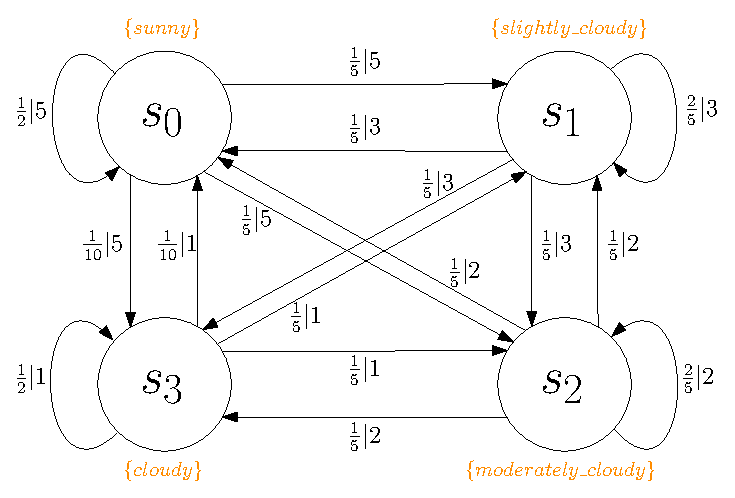
\includegraphics[width=0.5\linewidth]{resources/weather-solar-pannel}
    \captionsetup{justification=centering}
    \caption{MC modelling a daily production of energy (in $kJ$) of solar panels according to weather}
    \label{solarpanel}
  \end{figure}
  We are interested to know the probability that the weather suddenly goes from sunny to cloudy in at most three days
  (starting on a sunny day), i.e., $\mathbb{P}_{s_0}(\{s_0\} \U^{\leq 2} \{s_3\})$.
  Let $S_{=1} = \{s_3\}$ and $S_{=0} = \{ s_1, s_2 \}$, we have $S_? = \{s_0\}$. The least fixed point characterisation suggests the following iterative scheme:
  \begin{itemize}
    \item $x^{(0)} = 0$,
    \item $x^{(1)} = \Delta(s_0, s_0) \cdot x^{(0)} + \Delta(s_0, s_3) = \frac{1}{10},$ and
    \item $x^{(2)} = \Delta(s_0, s_0) \cdot x^{(1)} + \Delta(s_0, s_3) = \frac{1}{2} \cdot \frac{1}{10} + \frac{1}{10} = \frac{3}{20}$,
  \end{itemize}
  with $x^{(2)} = \mathbb{P}_{s_0}(\{s_0\} \U^{\leq 2} \{s_3\})$.
\end{example}
\begin{example}[\textit{Measuring constrained reachability event in an MC}] \label{constrained-reach-example}
Let $\mathcal{M}=(S, \Delta)$ be the MC of the figure \ref{CUTexample},
 $C = \{s_0, s_2, s_3\}$ and $T = \{s_1\}$. We are interested in the probability of the constrained reachability $C$ until $T$.
  \begin{figure}[H]
    \centering
    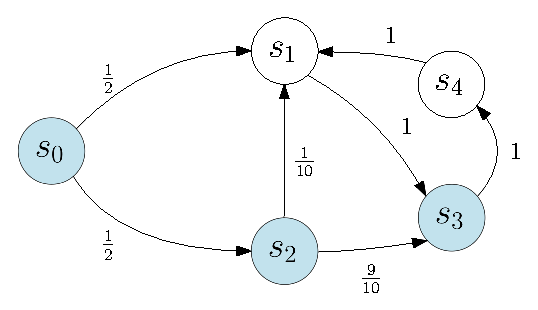
\includegraphics[width=0.4\linewidth]{resources/CUTexample}
    \captionsetup{justification=centering}
    \caption{MC $\mathcal{M}$ with state space $S = \{s_0, s_1, s_2, s_3, s_4\}$}\label{CUTexample}
  \end{figure}
  Let $S_{=1} = \{s_1\}$ and $S_{=0} = \{s \in S \; | \; \mathbb{P}_{s}(C\U T)=0\} = \{s_3, s_4\}$, we have $S_{?} = \{s_0, s_2\}$.
  The vector $(\mathbb{P}_{s}(C \U T))_{s \in S_?}$ is the unique solution of the following system:
  \begin{align*}
  	\begin{pmatrix}
      x_{s_0}\\[0.3em]
      x_{s_2}
  	\end{pmatrix} &=
    \begin{pmatrix}
      0 & \frac{1}{2} \\[0.3em]
      0 & 0
    \end{pmatrix}
    \begin{pmatrix}
      x_{s_0}\\[0.3em]
      x_{s_2}
    \end{pmatrix}
    +
    \begin{pmatrix}
      \frac{1}{2}\\[0.3em]
      \frac{1}{10}
    \end{pmatrix} \\
    \begin{pmatrix}
      x_{s_0}\\[0.3em]
      x_{s_2}
  	\end{pmatrix} &=
    \begin{pmatrix}
      \frac{1}{2} x_{s_2} \\[0.3em]
      0
    \end{pmatrix}
    +
    \begin{pmatrix}
      \frac{1}{2}\\[0.3em]
      \frac{1}{10}
    \end{pmatrix}
  \end{align*}
  So, $\mathbb{P}_{s_2}(C \U T) = x_{s_2} = \frac{1}{10}$ and $\mathbb{P}_{s_0}(C \U T) = x_{s_0} = \frac{11}{20}$.
  \\
\end{example}

With this background, we can finally introduce the following theorem.

\begin{theorem}[\textit{\textbf{Measurability of PCTL path formula events}}]
  Let $\mathcal{M}$ be an MDP with state space $S$, $s \in S$ be a state of $\mathcal{M}$ and $\phi$ be a PCTL path formula, the set $\{ \pi \in Paths(s) \; | \; \pi \models \phi \}$ is a measurable event.
\end{theorem}

\begin{proof2}
Let $Paths(s, \phi) = \{ \pi \in Paths(s) \; | \; \pi \models \phi \}$.
\begin{enumerate}
  \item If $\phi = \bigcirc \Phi$, then $Paths(s, \phi)$ agrees with the definition of $Cyl(ss')$, where $s' \models \Phi$.
  \item Else, if $\phi = \Phi_1 \U \Phi_2$, then the definition of
  $\pi \models \phi$ for any $\pi \in Paths(s)$ agrees with the definition of
  $\pi \models Sat(\Phi_1) \U Sat(\Phi_2)$.
  Thus, $Paths(s, \phi) = Sat(\Phi_1) \U Sat(\Phi_2)$.
  \item Else, if $\phi = \Phi_1 \U^{\leq n}\Phi_2$ for any $n \in \mathbb{N}$, then the definition of
  $\pi \models \phi$ for any $\pi \in Paths(s)$ agrees with the definition of
  $\pi \models Sat(\Phi_1) \U^{\leq n} Sat(\Phi_2)$.
  Thus, $Paths(s, \phi) = Sat(\Phi_1) \U^{\leq n} Sat(\Phi_2)$.
\end{enumerate}
As cylinder sets and constrained reachability events are measurable, $Paths(s, \phi)$ is measurable, for any path formula $\phi$.
\end{proof2}

\subsection{Limit behaviour}
Now, we will focus on events characterising the \textit{long-run} behaviour of Markov chains. We will address here two events : $\Box\Diamond T$ ($T$ is reached \textit{infinitely often})
and $\Diamond \Box T$ ($T$ is \textit{persistent}), for any subset of states $T \subseteq S$.
We will begin by defining these events and show that they are measurable. After that, we will introduce some graph theory notions, allowing to study the limit behaviour of Markov chains.
Studying the limit behaviour of Markov chains will allow to optimise
computations during the resolution of problems requiring linear equations systems or linear programs. Moreover, it will allow fast computations to determine probabilities of \textit{infinitely often} and \textit{persistent} events.

\begin{definition}[\textbf{Infinitely often event}]
  Let $\mathcal{M}=(S, \Delta, w, AP, L)$ be an MC, $T \subseteq S$, be a subset of states of $\mathcal{M}$, and
  $s \in S$ be a state of $\mathcal{M}$ from which events start. For any path $\pi = s_0 s_1 s_2 \dots \in Paths(s)$,
encountering \textit{infinitely often} $T$ actually means that, for all index $n \in \mathbb{N}$ (and thus, for any step $s_n$ of $\pi$), there exists an index $m \geq n$ such that $s_m \in T$. Then, let
  \begin{align*}
    Paths_{fin}^{m,\, T}(s) &= \{ s_0\dots s_m \in Paths_{fin}(s) \; | \; s_m \in T \}, \text{ and} \\
    Cyl^{m,\, T}(s) &= \bigcup_{s_0 \dots s_m \in Paths_{fin}^{m, \, T}(s)} Cyl(s_0\dots s_m)
  \end{align*}
  for any number of steps $m \in \mathbb{N}$. The infinitely often event for $T$ is defined as follows:
  \[
    \Box \Diamond T = \bigcap_{n \in \mathbb{N}} \bigcup_{m \geq n} Cyl^{m, \, T}(s).
  \]
  Since $\Box \Diamond T$ is formed by intersections of unions of cylinder sets, this event is measurable, and $\mathbb{P}_s(\Box\Diamond T)$ actually denotes the probability measure of this event, starting from the state $s \in S$.
\end{definition}

\begin{definition}[\textbf{Persistence event}]
  Let $\mathcal{M}=(S, \Delta, w, AP, L)$ be an MC, $T \subseteq S$, be a subset of states of $\mathcal{M}$, and
  $s \in S$ be a state of $\mathcal{M}$ from which events start. For any path $\pi = s_0 s_1 s_2 \dots \in Paths(s)$,
 $T$ is \textit{persistent} actually means there exists an index $n \in \mathbb{N}$ such that, for all $i\geq n$, $s_i \in T$. The persistence event for $T$ is defined as follows:
 \[
  \Diamond \Box T = \overline{\Box \Diamond (S \setminus T)}.
 \]
 Since $\Box \Diamond (S \setminus T)$ is measurable, $\Diamond \Box T$ is measurable, with \[\mathbb{P}_s(\Diamond \Box T) = 1 - \mathbb{P}_s(\Box \Diamond (S \setminus T)).\]
\end{definition}
We will now provide a way to compute the probability of these events with purely graph theory algorithms. To do that, we need to introduce some graph concepts.

\begin{definition}[\textbf{Bottom strongly connected components}]
Let $\mathcal{M}=(S, \Delta, w, AP, L)$ be an MC and $T \subseteq S$ be a subset of states of $\mathcal{M}$.
\begin{itemize}
  \item $T$ is \textit{strongly connected} if for any $s, s' \in T$, $s$ is connected to $s'$ in the underlying graph of $\mathcal{M}$, i.e., if there exists a finite path $s_0 \dots s_k \in Paths_{fin}(s)$ from $s$ to $s'$ in $\mathcal{M}$ such that $s_k = s'$.
  \item $T$ is a \textit{strongly connected component} (i.e., an \textbf{SCC}) of $\mathcal{M}$ iff $T$ is strongly connected and no proper superset of $T$ is strongly connected, i.e.,
  \[ T \text{ is strongly connected } \, \wedge \,
  \neg(\exists T', \; T' \text{ is strongly connected } \wedge \;
    T \subseteq T'). \]
  \item $T$ is a \textit{bottom strongly connected component} (i.e., a \textbf{BSCC}) of $\mathcal{M}$ iff
  $T$ is a SCC and no state outside $T$ can be reached, i.e.,
  \[
  T \text{ is an SCC} \; \wedge \; \forall s \in T, \,\Delta(s, T) = 1.
  \]
\end{itemize}
\end{definition}

SCCs and BSCCs of any Markov chain can be computed with
purely graph theory algorithms (e.g., with depth-first search algorithms based).

\begin{example}[\textit{Difference between SCCs and BSCCs}]
Let $\mathcal{M}=(S, \Delta)$ be the MC of the figure \ref{bsccex}. We have that the subset $T = \{s_1, s_2, s_3\} \subseteq S$ is an SCC because $T$ is the largest subset containing the state $s_1$ such that all states are connected to each other.
However, $T$ is not a BSCC because the state $s_3 \in T$ is connected by an edge in the underlying graph of $\mathcal{M}$ (we have $\Delta(s_3, s_4) > 0$), and $s_4$ is not connected to $T$.
Furthermore, the subset $B = \{s_5, s_6, s_7, s_8\} \subseteq S$ is a BSCC. Indeed, $B$ is the largest subset of $S$ containing $s_5$ such that all states are connected to each other. Moreover, each state $s \in B$ verify the following assertion:
$\Delta(s, B)=1$.
  \begin{figure}[h!]
    \centering
    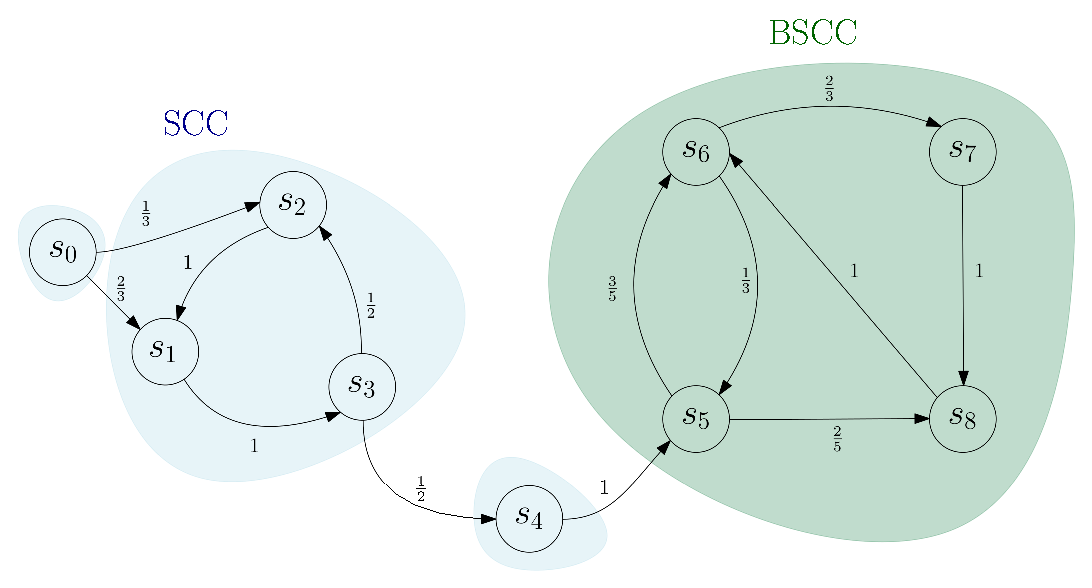
\includegraphics[width=0.7\linewidth]{resources/BSCC}
    \captionsetup{justification=centering}
    \caption{Markov chain $\mathcal{M}$ with state space composed by nine states, containing two SCCs and one BSCC}\label{bsccex}
  \end{figure}
\end{example}

\begin{theorem}[\textit{\textbf{Limit behaviour of Markov chains}}]\label{MCbehav}
Let $\mathcal{M}$ be an MC with state space $S$ and $s \in S$
be a state of $\mathcal{M}$ from which events start,
\[
  \mathbb{P}_s(\{\pi \in Paths(s) \; | \; inf(\pi) \text{ is a BSCC of }\mathcal{M}\}) = 1,
\]
where the $inf(\pi)$ denotes the set of states encountered infinitely often along $\pi = s_0 s_1 s_2 \dots \in Paths(s)$, i.e., $inf(\pi) = \{ s \in S \; | \; \forall n \in \mathbb{N},\, \exists m \geq n,\, s_m = s\}$.
\end{theorem}
A consequence of the theorem \ref{MCbehav} is that, starting from any state of a MC, the system ends up in a BSCC with probability one, and all states of this BSCC are visited infinitely often.

\begin{corollary}[\textbf{\textit{Quantitative repeated reachability}}]
  Let $\mathcal{M}$ be a finite MC with state space $S$, $T \subseteq S$ be a subset of states of $\mathcal{M}$, and $s \in S$ be a state of $\mathcal{M}$.
  Then, we can compute the probability to encounter infinitely often $T$ as follows:
  \[
    \mathbb{P}_s(\Box \Diamond T) = \mathbb{P}_s(\Diamond U),
  \]
  where $U$ is the union of all BSCCs $B$ of $\mathcal{M}$ such that $B \cap T \neq \emptyset$. Furthermore, we can compute the probability that $T$ is persistent as follows:
  \[
    \mathbb{P}_s(\Diamond \Box T) = \mathbb{P}_s(\Diamond U),
  \]
  where $U$ is the union of all BSCCs $B$ of $\mathcal{M}$ such that $B \subseteq T$.
\end{corollary}

\begin{proof2}
Let $BSCC(\mathcal{M})$ denotes the set of BSCCs of $\mathcal{M}$.
\begin{enumerate}
\item
Let $B \in BSCC(\mathcal{M})$ be a BSCC of $\mathcal{M}$.
In particular, let assume there exists a state $t \in T$ such that $t \in B$, then $\mathbb{P}_s(\Diamond B) = \mathbb{P}_s(\{ \pi \in Paths(s) \; | \; t \in inf(\pi) \; \wedge \; inf(\pi) = B \})$. Following the definition of BSCCs, we have that $B$ is the largest subset containing $t$ such that all states of $B$ are connected to each other and such that $\forall s' \in B, \, \Delta(s', B)=1$. Then, $B$ is the only BSCC containing $t$. So,
$\mathbb{P}_s(\Diamond B) = \mathbb{P}_s(\{ \pi \in Paths(s) \; | \; t \in inf(\pi)\}) = \mathbb{P}_s(\Box \Diamond \{t\})$,
by definition of $inf(\pi)$ and $\Box\Diamond \{t\}$.
\label{B1}
%\item Furthermore, let $t \in T$, it stills to show that if $\mathbb{P}_s(\Box \Diamond \{t\}) > 0$, then we always have that there exists a BSCC $B$ such that $\mathbb{P}_s(\Diamond B)>0$, $t \in B$. By contraposition, let assume that for all BSCC $B$ such that $\mathbb{P}_s(\Diamond B) > 0$, $t \centernot\in B$.
\item
Furthermore, let assume that for all BSCC $B$, $t \notin B$. As we have \[\mathbb{P}_s(\{\pi \in Paths(s)\; | \; t \notin inf(\pi), \, inf(\pi) \in BSCC(\mathcal{M})\}) = 1,\]
we obviously have $\mathbb{P}_s(\{\pi \in Paths(s)\; | \; t \in inf(\pi)\}) = 0$, i.e., $t$ is never visited infinitely often with a positive probability, and $\mathbb{P}_s(\Box\Diamond \{t\}) = 0$.
\label{B2}
\end{enumerate}
%A consequence of the theorem \ref{MCbehav} is that
%$\mathbb{P}_s(\Diamond \bigcup_{B \in BSCC(\mathcal{M})} B)
%= 1$. Then, there exists $B \in BSCC(\mathcal{M})$ such
%that $\mathbb{P}_s(\Diamond B) > 0$. If $t \in B$, then we
%have $\mathbb{P}_s(\Box\Diamond\{t\})>0$.
We can generalise \ref{B1} and \ref{B2} for all states in the set $T$:
\[\mathbb{P}_s(\Box \Diamond T) = \mathbb{P}_s(\Diamond \bigcup_{B \in BSCC(\mathcal{M}) \; | \; \exists t \in T, \, t \in B } B)\]
The second assertion can be shown in a similar way.
%\vspace{-0.1\linewidth}
\end{proof2}\\

Now, we will come back on a problem addressed previously in the remark \ref{remarkS0S1}. Indeed, following an MC $\mathcal{M}$ with state space $S$ and two subsets $C, T \subseteq S$, we have presented a graph theory based solution to compute the largest subset $S_{=0}$, i.e., $\{s \in S \; | \; \mathbb{P}_s(C \U T) = 0\}$, but we have not yet presented a solution to compute the largest subset $S_{=1}$, i.e., $\{s \in S \; | \; \mathbb{P}_s(C \U T) = 1\}$.
We will see that qualitative properties can be verified thanks to the notion of BSCC.

\begin{notation}[\textit{Absorbing state}]
  Let $\mathcal{M}=(S, \Delta, w, AP, L)$ be an MC and $s \in S$ be a state of $\mathcal{M}$. We say that $s$ is absorbing iff $\Delta(s, s') = 1$.
\end{notation}

\begin{theorem}[\textbf{\textit{Almost sure reachability}}]\label{asr}
  Let $\mathcal{M}$ be a finite MC with state space $S$, $s \in S$ be a state of $\mathcal{M}$ from which events start, $T \subseteq S$ be a set of absorbing states, and the two following successors and predecessors sets:
\begin{align*}
  Succ^*(s) &= \{ s' \in S \; | \; \exists \pi = s_0s_1s_2\dots \in Paths(s) \;\; \exists k \in \mathbb{N}_0, \, s_k = s' \}, \\
  Pred^*(T) &= \{ s' \in S \; | \; \exists \pi = s_0s_1s_2\dots \in Paths(s')\; \exists k \in \mathbb{N}_0, \, s_{k} \in T \,\}.
\end{align*}
   Then , the following statements are equivalent:
  \begin{enumerate}[(a)]
    \item $\mathbb{P}_s(\Diamond T)= 1$. \label{succ1}
    \item $Succ^*(s') \cap T \neq \emptyset, \; \forall s' \in Succ^*(s)$.\label{succ2}
    \item $s \in S \setminus Pred^*(S \setminus Pred^*(T))$. \label{succ3}
  \end{enumerate}
  In particular, \[
  \{s \in S \; | \; \mathbb{P}_s(\Diamond T) = 1\} =
  S \setminus Pred^*(S \setminus Pred^*(T))
  \]
  \begin{figure}[h]
  \centering
  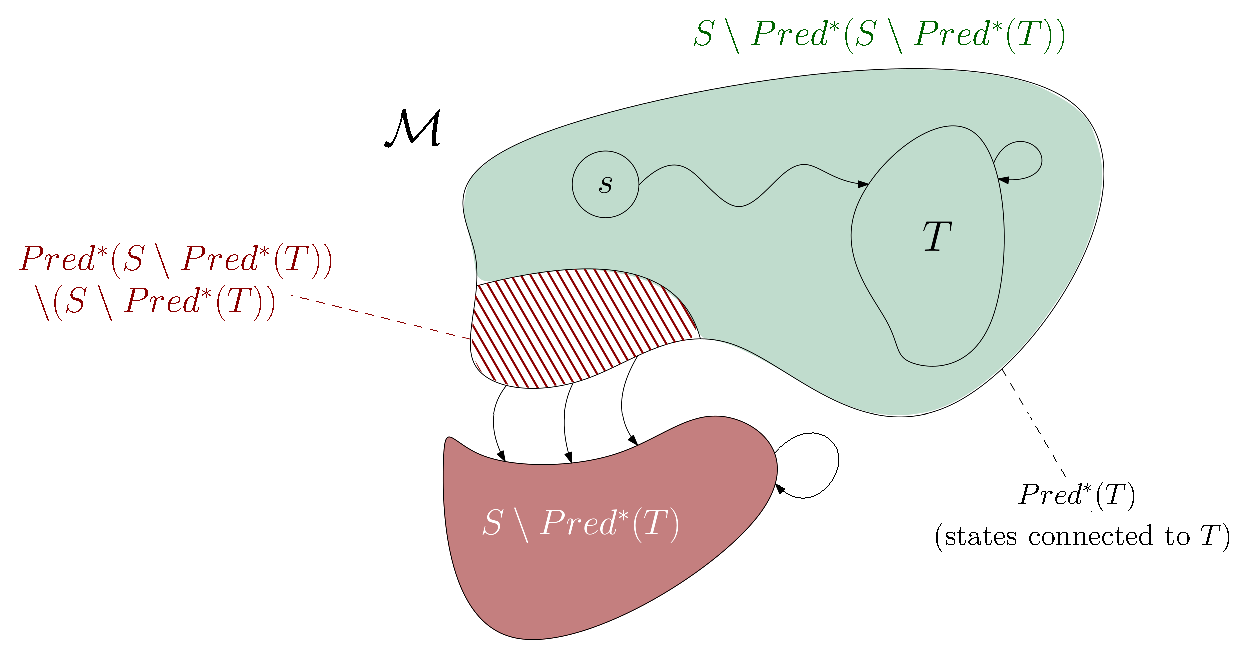
\includegraphics[width=0.8\linewidth]{resources/S1BSCC}
  \caption{Intuitive representation of the subset $S \setminus Pred^*(S \setminus Pred^*(T))$}\label{spred}
  \end{figure}
\end{theorem}
\begin{proof2}\cite{PMC}
We can easily derivate from the definitions of the sets $Succ^*$ and $Pred^*$ that \ref{succ2} and \ref{succ3} are equivalent. \\
($\neg\ref{succ2}\implies\neg\ref{succ1}$). Let $s' \in Succ^*(s)$ such that $Succ^*(s') \cap T = \emptyset$ Following the figure \ref{spred}, we have that $s$ is in the subset represented by a red tiling pattern or $s$ is in the red subset and we have that $s'$ is in the red subset. Thus, $s'$ is a successor of $s$ from which $T$ can not be reached. Then, we have $\mathbb{P}_s(\Diamond T) \leq 1 - \mathbb{P}_s(\Diamond \{s'\}) < 1$.
%Furthermore, referring the figure
%\ref{spred}, we have that $1 - \mathbb{P}_s(\Diamond T) = \mathbb{P}_s(\Diamond (S \setminus Pred^*(T)))$.\\
($\ref{succ2} \implies \ref{succ1}$). Let assume that $Succ^*(s') \cap T \neq \emptyset$, for any successor $s'$ of $s$. By the theorem \ref{MCbehav}, we reach a BSCC from $s$ with a probability one. Since each state in $t \in T$ is absorbing, each BSCC $B$ of $\mathcal{M}$ consists in $B = \{t\}$ or it satisfies $T \cap B = \emptyset$. We will show that the latter case can not occur from $s$.
Consider $T \cap B = \emptyset$ for BSCC $B$.
As $B$ is a BSCC, $Succ^*(u)\cap T = \emptyset$, for each $u \in B$.
However, as $T$ is reachable for any $s' \in Succ^*(s)$, there is no BSCC with $T \cap B = \emptyset$ that is reachable from $s$. So, we almost surely have a state in $T$ that will be reached from the state $s$.
\end{proof2}
\\

The theorem \ref{asr} allows to compute the largest subset $S_{=1} = \{s \in S \; | \; \mathbb{P}_s(\Diamond T) = 1 \}$ for any finite MC with state space $S$ and for any $T \subseteq S$ as follows:
%Indeed, we begin by make all states in $T$ absorbing. This allows to apply the theorem \ref{asr}.
%Then, we can compute all states connected
\begin{algorithm}[H]
\caption{Almost sure reachability}\label{almost-sure-algo}
\begin{algorithmic}[1]
  \REQUIRE a finite Markov chain $\mathcal{M}$ with state space $S$, a transition function $\Delta$, and a set of target states $T \subseteq S$.
  \ENSURE the set $\{ s \in S \; | \; \mathbb{P}_s(\Diamond T) = 1\}$.
  \item[]
  \STATE $\Delta_T \leftarrow \lambda (s, s'):\, \begin{cases}
    1 &\text{if } s = s' \text{ and } s \in T\\
    \Delta(s, s') &\text{else}
  \end{cases}$
  \STATE $\mathcal{M}_T \leftarrow (S, \Delta_T)$
  \COMMENT{make all states of $T$ absorbing, yielding a new MC $\mathcal{M}_T$}
  \STATE $Pre^*(T) \leftarrow \mathsf{backward\_search}(G^{\mathcal{M}_T}, T)$
  \COMMENT{compute the set of states connected to $T$}
  \STATE $Pre^*(S \setminus Pre^*(T)) \leftarrow \mathsf{backward\_search}(G^{\mathcal{M}_T}, S \setminus Pre^*(T))$
  \RETURN $S \setminus Pre^*(S \setminus Pre^*(T))$
\end{algorithmic}
\end{algorithm}
\noindent where the notation $\lambda x:y$ is a lambda calculus based notation that gives the lambda calculus expression $\lambda x.y \equiv x \mapsto y$, $G^\mathcal{M}$ denotes the underlying graph of $\mathcal{M}$ and the $\mathsf{backward\_search}$ algorithm
, for inputs $G^{\mathcal{M}_T}$ and $T$, explores $G^{\mathcal{M}_T}$ from the set $T$: it starts by marking all states of $T$, and then iteratively marks all unmarked predecessors of marked states (\textit{backward breadth-first search}). All marked states are thus connected to $T$. An alternative recursive version of this algorithm exists (\textit{backward depth-first search}).
The time complexity of this algorithm is in $\mathcal{O}(|\mathcal{M}_T|)$.

\begin{corollary}[\textbf{\textit{Qualitative constrained reachability}}] Let $\mathcal{M}$ be a finite MC with state space $S$ and $C, T \subseteq S$, the sets
\[
  S_{=0} = \{ s \in S \; | \; \mathbb{P}_s (C \U T) = 0 \} \text{ and } S_{=1} = \{ s \in S \; | \; \mathbb{P}_s (C \U T ) = 1 \}
  \]
  can be computed in time $\mathcal{O}(|\mathcal{M}|)$.
\end{corollary}
\begin{proof2}\cite{PMC}
\begin{enumerate}
  \item We can determine $S_{=0}=\{s \in S \; | \; \mathbb{P}_s(C \U T)=0\}$ by computing the complement of the set $\{s \in S \; | \; \exists \pi \in Paths(\pi), \, \pi \models C \U T \}$ (cf. lemma \ref{S0graph}).
  \item A linear-time algorithm for the computation of $S_{=1}=\{ s\in S \; | \; \mathbb{P}_s(C \U T) = 1 \}$ can be solved by a reduction to the reachability problem to $T$ in a slightly modified MC. The idea is the following: we make all states of $T$ absorbing (to take advantage of the theorem \ref{asr}) and do the same for all states in $S \setminus (C \cup T)$.
  The probability transition function of this modified MC $\mathcal{M}'$ is
  defined as follows:
  \[
    \Delta'(s, s') = \begin{cases}
      1 & \text{if } s=s' \text{ and } s'\in T \cup S \setminus(C \cup T),\\
      0 & \text{if } s \neq s' \text{ and } s \in T \cup S \setminus (C \cup T),\, \text{and}\\
      \Delta(s, s') & \text{otherwise}.
    \end{cases}
  \]
  Thus, we have:
  \begin{itemize}
    \item $\mathbb{P}_s^\mathcal{M}(C \U T) = \mathbb{P}_s^\mathcal{M'}(\Diamond T)$ for all states $s \in C \setminus T$,
    \item $\mathbb{P}_s^\mathcal{M}(C \U T) = \mathbb{P}_s^{\mathcal{M}'}(\Diamond T) = 1$
    for all states $s \in T$, and
    \item $\mathbb{P}_s^\mathcal{M}(C \U T)= \mathbb{P}_s^{\mathcal{M}'}(\Diamond T) = 0$ for all states $s \in S \setminus (C \cup T)$.
  \end{itemize}
  Doing this reduction, we can now apply the lemma \ref{S0graph} on $\mathcal{M}'$ to compute the largest set $S_{=0}$. Since $\Diamond T = S \U T$, we have $S_{=0}= S \setminus Pred^*(T)$. Then, we can apply the theorem  \ref{asr} to compute the largest set $S_{=1}$ with the algorithm \ref{almost-sure-algo}.
\end{enumerate}
\end{proof2}\\

Thus, check if each temporal events presented in this section holds with a probability one or zero can be done through simple graph theory algorithms in $\mathcal{O}(|\mathcal{M}|)$, without referring to probabilities of transitions.

\section{PCTL model checking}
\begin{definition}[\bfseries PCTL model checking]
Let $\mathcal{M}$ be an MC with state space $S$, $s \in S$ be a state of $\mathcal{M}$, and $\Phi$ be a PCTL state formula. The model checking problem for $\mathcal{M}$, $s$ and $\Phi$ consists of deciding if $s \models \Phi$, i.e., if $s \in Sat(\Phi)$.
\end{definition}
Following an MC $\mathcal{M}$, a state $s$ of this MC and a state formula $\Phi$, determine if $s \models \Phi$ can be done through a bottom-up traversal of the \textit{parse tree} of $\Phi$.
Indeed, according to the PCTL syntax, we recursively decompose $\Phi$ following its sub-formulae. Moreover, each sub-formula of $\Phi$ is actually represented by a node of this tree. For each PCTL state formula $\Phi$, we compute its satisfaction set from the node representing the formula, according to each satisfaction set computed from each of its child and the characterisation of $Sat(\Phi)$.
\begin{property}[Characterisation of Sat]
Let $\mathcal{M} = (S, \Delta, w, AP, L)$ be an MC, $\Phi, \Psi$ be PCTL state formulae over $AP$, and $\phi$ be a  PCTL path formula over $AP$. The satisfaction set $Sat$ is characterised as follows:
\begin{flalign*}
  Sat(true) &= S,\\
  Sat(a) &= \{s \in S \; | \; a \in L(s)\} \text{ for } a \in AP,\\
  Sat(\Phi) \, \wedge \, Sat(\Psi) &= Sat(\Phi) \cap Sat(\Psi),\\
  Sat(\neg \Phi) &= S \setminus Sat(\Phi), \text{ and} \\
  Sat(\mathcal{P}_J(\phi)) &= \{ s \in S \; | \; \mathbb{P}_s (Paths(s, \phi)) \in J \} \text{ for } J \subseteq [0, 1],
\end{flalign*}
where $Paths(s, \phi) = \{ \pi \in Paths(s) \; | \; \pi \models \phi \}$.
$\mathcal{P}_J(\phi)$ is computed according to the formula $\phi$ as follows:
let $s \in S$ be a state of $\mathcal{M}$,
\begin{flalign*}
  \mathbb{P}_s(Paths(s,\, \bigcirc \Phi)) &= \sum_{s' \in Sat(\Phi)} \Delta(s, s'), \\
  \mathbb{P}_s(Paths(s,\, \Phi \U \Psi)) &= \mathbb{P}_s(Sat(\Phi) \U Sat(\Psi)), \text{ and}\\
  \mathbb{P}_s(Paths(s, \, \Phi \U^{\leq n} \Psi)) &=
    \mathbb{P}_s(Sat(\Phi) \U^{\leq n} Sat(\Psi)). \tag{cf. section \ref{tempevent}}
\end{flalign*}
Additionally, we can optimise the computation of the satisfiability sets of the following formulae:
\begin{align*}
  Sat(\mathcal{P}_J(\Diamond \mathcal{P}_{=1} (\Box \mathcal{P}_{=1}(\Diamond a)))) &=
\{ s \in S \; | \; \mathbb{P}_s (\Box \Diamond Sat(a)) \in J \}, \tag{\textit{\small infinitely often}} \\
Sat(\mathcal{P}_J(\Diamond \mathcal{P}_{=1}(\Box a))) &= \{ s \in S \; | \; \mathbb{P}_s(\Diamond \Box Sat(a)) \in J\}, \tag{\textit{persistence}}
\end{align*}
for $J \subseteq [0, 1]$ and $a \in AP$.
\end{property}

\begin{example}[\textit{PCTL model checking of an MC via its parse tree}]
  Let $\mathcal{M}=(S, \Delta, w, AP, L)$ be the MC of the figure \ref{CUTexample2} and the state formula $\Phi = c \vee \mathcal{P}_{\geq \frac{1}{2}}(a \U (b \wedge c))$.
  \begin{figure}[h!]
  \begin{minipage}{0.4\linewidth}
    \centering
    \includegraphics[width=\linewidth]{resources/CUTexample2}
    \captionsetup{justification=centering}
    \captionof{figure}{MC $\mathcal{M}$ with state space $S = \{s_0, s_1, s_2, s_3, s_4\}$ and atomic propositions of the set $AP = \{a, b, c\}$}
    \label{CUTexample2}
  \end{minipage}
    $ \quad $
  \begin{minipage}{0.6\linewidth}
    \centering
    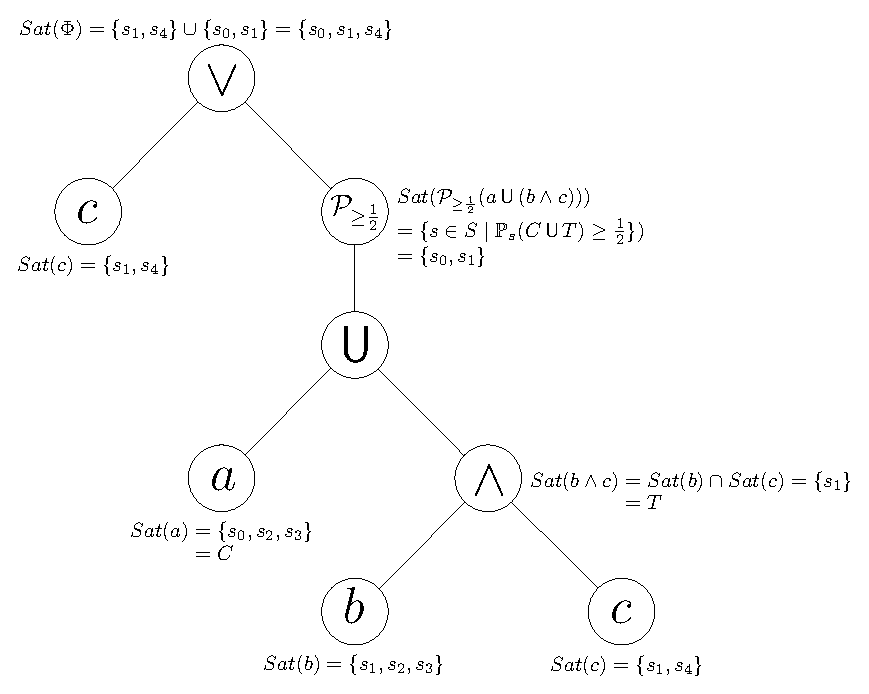
\includegraphics[width=\linewidth]{resources/parse-tree}
    \captionsetup{justification=centering}
    \captionof{figure}{Parse tree of $\mathcal{M}$ for $\Phi$}
    \label{parse-tree-example}
  \end{minipage}
  \end{figure}
  We are interested to know if $s_0 \models \Phi$. To do that, we build the parse tree of $\Phi$.
  This one is given in the figure \ref{parse-tree-example}. We can compute $Sat(\Phi)$ through a bottom up traversal of this tree: we begin at the leaves of the tree, i.e., by computing $Sat(a)$, $Sat(b)$, and $Sat(c)$. Then, we compute $Sat(b \wedge c)$, that equals $Sat(b)\cap Sat(c)$, according to the characterisation of the satisfaction set.
  After that, we compute
  $Sat(\mathcal{P}_{\geq \frac{1}{2}}(a \U (b \wedge c)))$ by computing $\{ s \in S \; | \; \mathbb{P}_s(Sat(a) \U Sat(b \wedge c)) \geq \frac{1}{2}\} = \{ s \in S \; | \; \mathbb{P}_s(\{s_0, s_2, s_3\} \U \{s_1\}) \geq \frac{1}{2}\}$.
  We actually have already computed these probabilities (cf. example \ref{constrained-reach-example}).
  So, this set equals $\{ s_0, s_1 \}$.
  Finally, since we have already computed $Sat(c)$ and $Sat(\mathcal{P}_{\geq \frac{1}{2}}(a \U (b \wedge c)))$, we can compute $Sat(\Phi) = \{s_1, s_4\} \cup \{s_0, s_1\} = \{s_0, s_1, s_4\}$.
  As $s_0 \in Sat(\Phi)$, then $s_0 \models \Phi$.
\end{example}

\section{PCTL for Markov decision processes}
The PCTL syntax for MDPs is exactly the same as for MCs with the exception of the probabilistic operator $\mathcal{P}_J(.)$ due to the nondeterminism of MDPs:
we can not verify probabilistic properties without referring to the notion of strategy.
Then, we replace this operator with $\mathcal{P}^{\max}_J(.)$, referring to the strategy offering the maximum probability of satisfying a given property.
Thus, the formula $\mathcal{P}^{\max}_J(\phi)$ asserts \[\mathbb{P}^{\max}_s(\{\pi \in Paths(s) \; | \; \pi \models \phi \}) \in J .\]
\textit{Note: remind that $\mathbb{P}_s^{\max}(E)$ refers to the probability measure defined on the MC induced by the strategy maximising the probability of the event $E$ in this MC, i.e., $\max_{\sigma} \mathbb{P}_s^\sigma(E)$.}

\begin{definition}[\textbf{Syntax of PCTL for MDPs}]
Let $AP$ be a set of atomic propositions,
\begin{itemize}
  \item PCTL \textit{state formulae} are formed according the following grammar:
  \[
    \Phi ::= true \;\; | \;\; a \;\; | \;\; \Phi_1 \wedge \Phi_2 \;\; | \;\; \neg \Phi \;\; | \;\; \mathcal{P}^{\max}_J(\phi)
  \]
  where $a \in AP$ is an atomic proposition, $J \subseteq [0, 1]$ gives probability bounds and $\phi$ is a path formula.
  \item PCTL \textit{path formulae} are formed according
  to the same grammar than for MCs.
\end{itemize}
\end{definition}
\begin{definition}[\textbf{Semantic of PCTL for MDPs}]
  Let $\mathcal{M} = (S, A, \Delta, AP, L)$ be an MDP and $s \in S$, be a state of $\mathcal{M}$,
  \begin{flalign*}
  \intertext{$s \models \Phi$ iff the state formula $\Phi$ holds in the state $s$, i.e.,}
    &\bigcdot\; s \models true, &&&\\
    &\bigcdot\; s \models a &\text{ iff }& a \text{ is a label of $s$, i.e., } a \in L(s),&\\
    &\bigcdot\; s \models \Phi_1 \wedge \Phi_2&\text{ iff }& s \models \Phi_1 \text{ and } s \models \Phi_2,&\\
    &\bigcdot\; s \models \neg \Phi &\text{ iff }& s \not\models \Phi, &\\
    &\bigcdot\; s \models \mathcal{P}^{\max}_J(\phi) &\text{ iff }& \mathbb{P}^{\max}_s(\{ \pi \in Paths(s) \; | \; \pi \models \phi \}) \in J.&
  \intertext{$\pi \models \phi$ iff the $\pi$ satisfies $\phi$ in the induced MC.}
  \end{flalign*}
\end{definition}
In the first chapter, we have addressed a way to compute the strategy $\sigma$ to resolve the SR problem, i.e., compute the strategy $\sigma$ following an MDP $\mathcal{M}$ with state space $S$, a state $s \in S$, and a subset of target states $T$, such that $\mathbb{P}_s^\sigma(\Diamond T) = \mathbb{P}^{\max}_s(\Diamond T)$.
We have seen that this can be done in polynomial time in the size of $\mathcal{M}$, through a linear program (cf. theorem \ref{thm-sr} and appendix \ref{app-sr}).
We can generalise this computation of optimal strategy for the constrained reachability events. To this purpose, we need to address the equation system from which the linear program used to compute this strategy is derived (cf. appendix \ref{app-sr}).

\begin{theorem}[\textbf{Equation system for max reachability probabilities}]
  Let $\mathcal{M}$ be a finite MDP with state space $S$ and with a probability transition function $\Delta$, $s \in S$ be a state of $\mathcal{M}$ and $T \subseteq S$ be a subset of target states. The vector $(x_s)_{s \in S}$ with $x_s = \mathbb{P}_s^{\max}(\Diamond T)$ yields the unique solution of the following equation system: let the subset $S_{=1} \subseteq S$ be a subset of states such that $T \subseteq S_{=1} \subseteq \{s \in S \; | \; \mathbb{P}^{\max}_s(\Diamond T) = 1 \}$,
  \begin{itemize}
    \item if $s \in S_{=1}$, then $x_s=1$,
    \item else if $s$ is not connected to $T$ in the underlying graph of $\mathcal{M}$, then $x_s=0$,
    \item else,
    \[ x_s = \max_{\alpha \in A(s)} \sum_{s' \in Succ(s, \alpha)} \Delta(s, \alpha, s') \cdot x_{s'}. \]
  \end{itemize}
\end{theorem}
This theorem suggests an iterative approximation technique, called \textit{value iteration}, to compute the values $x_s=\mathbb{P}^{\max}_s(\Diamond T)$. First, we fix the values of $x_s^{(n)} = x_s$, for all $n \in \mathbb{N}$, according to the two first conditions of the equation system by a backward reachability analysis of the underlying graph of $\mathcal{M}$. For other states $s$, we have
\[x_s = \lim_{n \rightarrow \infty} x_s^{(n)}\]
where
\[x_s^{(0)} = 0 \quad \text{and} \quad x_s^{(n+1)} = \max_{\alpha \in A(s)} \sum_{s' \in Succ(s, \alpha)} \Delta(s, \alpha, s') \cdot x_{s'}^{(n)}. \]
This yields $x_s^{(n)} \leq x_s^{(n+1)}$ for any $n \in \mathbb{N}$, and the values of $\mathbb{P}^{\max}_s(\Diamond T)$ can be approximated by iteratively computing vectors $x_s^{(n+1)}$
with vectors $x_s^{(n)}$ for all states $s \in S$ until $\max_{s \in S} |x_s^{(n+1)} - x_s{(n)}| < \varepsilon$ for a small threshold value $\varepsilon > 0$.
\begin{theorem}[\textbf{Value iteration for step-bounded reachability}]
  Let $\mathcal{M}$ be a finite MDP with state space $S$ and with a probability transition function $\Delta$, and a subset of target states $T \subseteq S$. The value iteration approach can be used to compute the maximal probabilities for the event $\Diamond^{\leq n}T$.
  Indeed, the vector $(x_s)^{(n)}_{s \in S}$ with $x_s^{(n)} = \mathbb{P}^{\max}_s(\Diamond^{\leq n} T)$ yields the unique solution of the following equation system:
  \begin{itemize}
    \item if $s \in T$, then $x_s^{(n)}=1$ for all $n \in \mathbb{N}$,
    \item else if $s$ is not connected to $T$ in the underlying graph of $\mathcal{M}$, then $x_s^{(n)}=0$
    for all $n \in \mathbb{N}$,
    \item else, $x_s^{(0)} = 0$ and
    \[ x_s^{(n+1)} = \max_{\alpha \in A(s)} \sum_{s' \in Succ(s, \alpha)} \Delta(s, \alpha, s') \cdot x_{s'}^{(n)}. \]
  \end{itemize}
  According to this equation system, we can build a finite memory strategy $\sigma = (Q, \sigma_\alpha, \delta, \delta_0)$ such that $\mathbb{P}^\sigma_s(\Diamond^{\leq n} T) = \mathbb{P}^{\max}_s(\Diamond^{\leq n} T)$ for $s \in S$ and $n \in \mathbb{N}$:
  assume that modes of $Q$ range from $0$ to $n$ such that $\delta_0(s) = m_0$ and $\delta(m_i, s) = m_{\min\{i+1, n\}}$ for all $s \in S$ and $i \in \{0, \dots, n\}$. Then, we define $\sigma_\alpha$ as follows:
  \[
    \sigma_\alpha(m_i, s) =
    \begin{cases}
      \alpha \; \text{ such that } \alpha \in A(s) &\text{if }i=0,\\
      \arg \max_{\alpha \in A(s)} \sum_{s' \in Succ(s, \alpha)} \Delta(s, \alpha, s') \cdot x_{s'}^{(i-1)}
      & \text{else.}
    \end{cases}
  \]
  Intuitively, $\sigma$ is initialised in mode $m_0$, and when the strategy is in mode $m_i$, $i \in \{1, \dots, n-1\}$,
  it chooses the action that maximises $\sum_{s' \in Succ(s, \alpha)} \Delta(s, \alpha, s') \cdot x_{s'}^{(i-1)}$ and then changes its mode $m_i$ to the next mode $m_{i+1}$. When the strategy is in mode $m_n$, it stays inside it forever.
\end{theorem}
As for MCs, we can compute constrained reachability events $C \U T$ or $C \U^{\leq n} T$ by reduction to the reachability to $T$ as follows:
we make all states of $s \in S \setminus (C \cup T)$ absorbing i.e., we replace all the enabled actions of $A(s)$
by an unique action $\alpha_s$ such that $\Delta(s, \alpha_s, s) = 1$.
Then, we compute $\mathbb{P}^{\max}_s(\Diamond T)$ in this modified MDP to get the linked strategy.
